\documentclass{standalone}
\usepackage[dvipsnames]{xcolor}{}
\usepackage{tikz}
\newcommand{\drawMineUnvisited}[1]{\draw [lightgray, fill=lightgray, fill opacity=0.5] #1 circle [radius=0.4]}
\newcommand{\drawMineFrontier}[1]{\draw [SkyBlue, fill=SkyBlue, fill opacity=0.5] #1 circle [radius=0.4]}
\newcommand{\drawMineVisited}[1]{\draw [orange, fill=orange, fill opacity=0.5] #1 circle [radius=0.4]}
\newcommand{\drawMineFound}[1]{\draw [green, fill=green, fill opacity=0.5] #1 circle [radius=0.4]}
\newcommand{\drawMineNotFound}[1]{\draw [black, fill=black, fill opacity=0.9] #1 circle [radius=0.4]}


\begin{document}
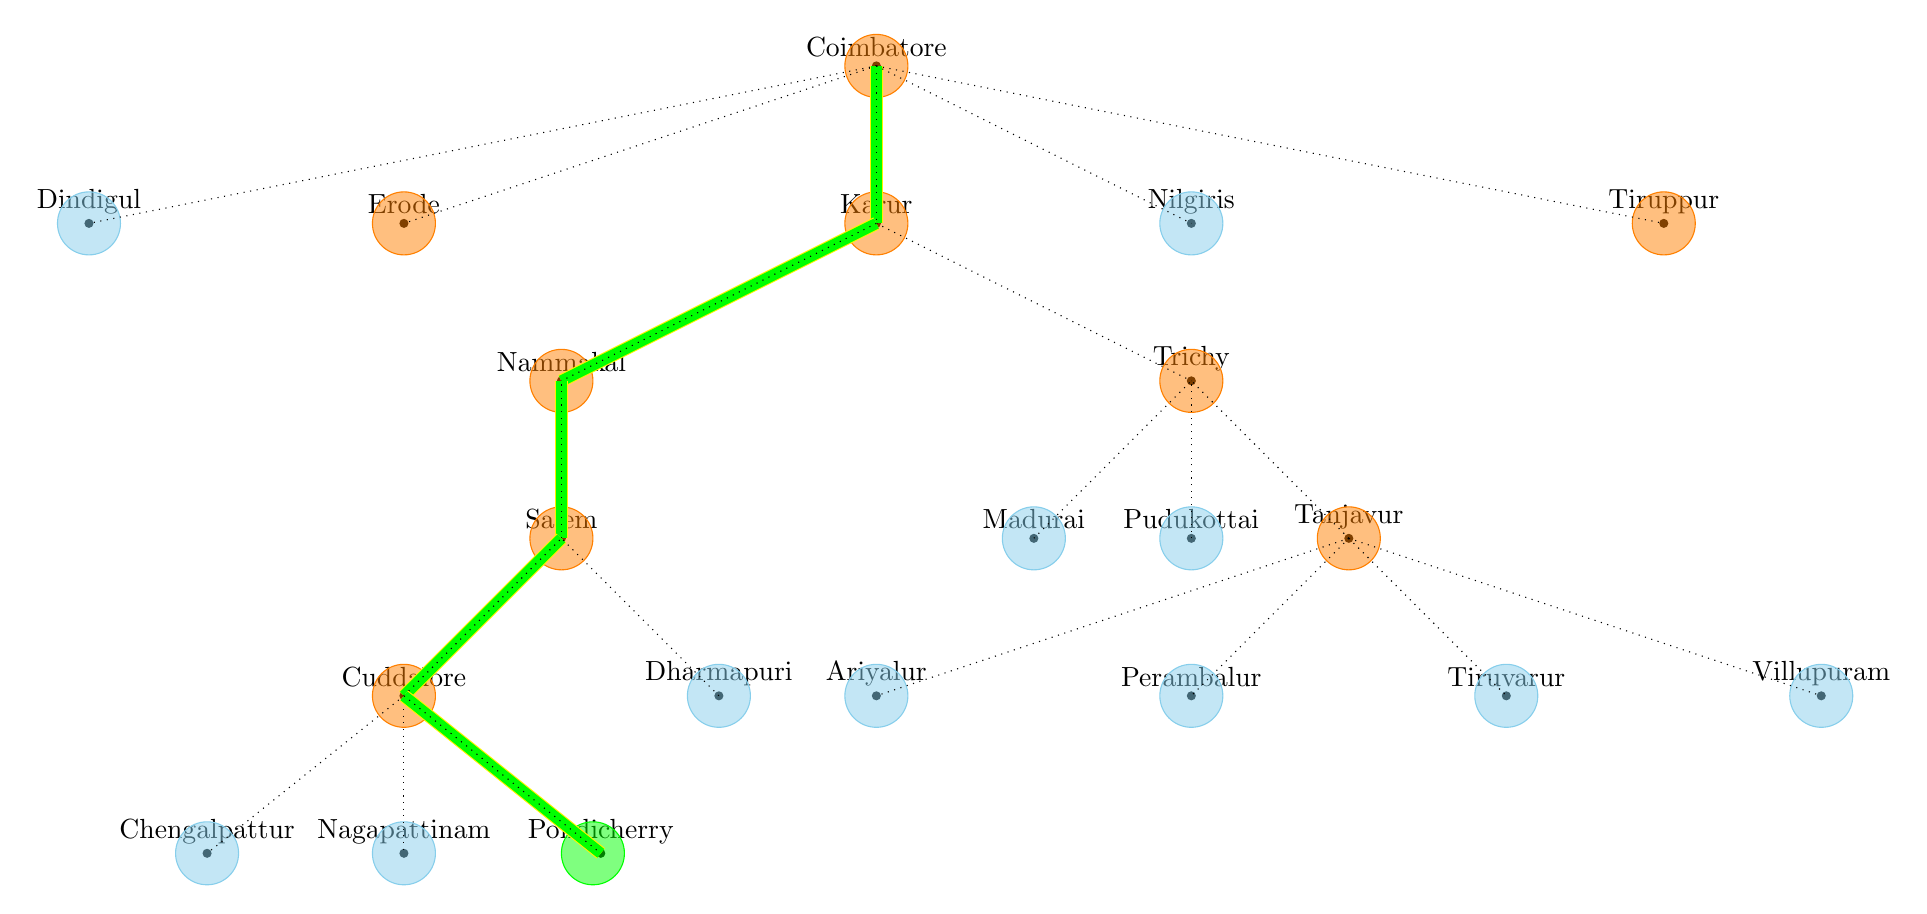
\begin{tikzpicture}
    \draw [black, fill=black ] (-0,0) circle [radius=0.05] node[above] {Coimbatore};
    \drawMineVisited{(-0,0)};

    %for coimbatore
    \draw [fill=black] (-6,-2) circle [radius=0.05] node[above] {Erode};
    \drawMineVisited{(-6,-2)};
    \draw [ dotted] (-0,0) -- (-6,-2);

    \draw [fill=black] (-10,-2) circle [radius=0.05] node[above] {Dindigul};
    \drawMineFrontier{(-10,-2)};
    \draw [ dotted] (-0,0) -- (-10,-2);

    \draw [fill=black] (0,-2) circle [radius=0.05] node[above] {Karur};
	\drawMineVisited{(-0,-2)};
    \draw [ dotted, preaction={%But before that
    draw,yellow,-,% Draw yellow without any arrow head
    double=green,
    double distance=10\pgflinewidth,
    }] (-0,0) -- (-0,-2);

    \draw [fill=black] (4,-2) circle [radius=0.05] node[above] {Nilgiris};
	\drawMineFrontier{(4,-2)};
    \draw [ dotted] (-0,0) -- (4,-2);

    \draw [fill=black] (10,-2) circle [radius=0.05] node[above] {Tiruppur};
	\drawMineVisited{(10,-2)};
    \draw [ dotted] (-0,0) -- (10,-2);

    % for Karrur
    \draw [fill=black] (4,-4) circle [radius=0.05] node[above] {Trichy};
	\drawMineVisited{(4,-4)};
    \draw [ dotted] (0,-2) -- (4,-4);

    \draw [fill=black] (-4,-4) circle [radius=0.05] node[above] {Nammakal};
	\drawMineVisited{(-4,-4)};
    \draw [ dotted, preaction={%But before that
    draw,yellow,-,% Draw yellow without any arrow head
    double=green,
    double distance=10\pgflinewidth,
    }] (0,-2) -- (-4,-4);

    % for Nammakal
    \draw [fill=black] (-4,-6) circle [radius=0.05] node[above] {Salem};
     \drawMineVisited{(-4,-6)};
     \draw [ dotted, preaction={%But before that
     draw,yellow,-,% Draw yellow without any arrow head
     double=green,
     double distance=10\pgflinewidth,
     }] (-4,-6) -- (-4,-4);



     % for Trichy
     \draw [fill=black] (2,-6) circle [radius=0.05] node[above] {Madurai};
     \drawMineFrontier{(2,-6)};
     \draw [ dotted] (2,-6) -- (4,-4);

     \draw [fill=black] (4,-6) circle [radius=0.05] node[above] {Pudukottai};
     \drawMineFrontier{(4,-6)};
     \draw [ dotted] (4,-6) -- (4,-4);

     \draw [fill=black] (6,-6) circle [radius=0.05] node[above] {Tanjavur};
     \drawMineVisited{(6,-6)};
     \draw [ dotted] (6,-6) -- (4,-4);

     % for Tanjarvur
     \draw [fill=black] (0,-8) circle [radius=0.05] node[above] {Ariyalur};
     \drawMineFrontier{(0,-8)};
     \draw [ dotted] (6,-6) -- (0,-8);

     \draw [fill=black] (4,-8) circle [radius=0.05] node[above] {Perambalur};
     \drawMineFrontier{(4,-8)};
     \draw [ dotted] (6,-6) -- (4,-8);

     \draw [fill=black] (8,-8) circle [radius=0.05] node[above] {Tiruvarur};
     \drawMineFrontier{(8,-8)};
     \draw [ dotted] (6,-6) -- (8,-8);

     \draw [fill=black] (12,-8) circle [radius=0.05] node[above] {Villupuram};
     \drawMineFrontier{(12,-8)};
     \draw [ dotted] (6,-6) -- (12,-8);

     % for Salem
     \draw [fill=black] (-6,-8) circle [radius=0.05] node[above] {Cuddalore};
     \drawMineVisited{(-6,-8)};
     \draw [ dotted, preaction={%But before that
     draw,yellow,-,% Draw yellow without any arrow head
     double=green,
     double distance=10\pgflinewidth,
     }] (-6,-8) -- (-4,-6);

     \draw [fill=black] (-2,-8) circle [radius=0.05] node[above] {Dharmapuri};
     \drawMineFrontier{(-2,-8)};
     \draw [ dotted] (-2,-8) -- (-4,-6);

     % for Cuddalore
     \draw [fill=black] (-8.5,-10) circle [radius=0.05] node[above] {Chengalpattur};
     \drawMineFrontier{(-8.5,-10)};
     \draw [ dotted] (-6,-8) -- (-8.5,-10);

     \draw [fill=black] (-6,-10) circle [radius=0.05] node[above] {Nagapattinam};
     \drawMineFrontier{(-6,-10)};
     \draw [ dotted] (-6,-8) -- (-6,-10);
    

     \draw [fill=black] (-3.5,-10) circle [radius=0.05] node[above] {Pondicherry};
     \drawMineFound{(-3.6,-10)};
     \draw [ dotted, preaction={%But before that
     draw,yellow,-,% Draw yellow without any arrow head
     double=green,
     double distance=10\pgflinewidth,
     }] (-6,-8) -- (-3.5,-10);

     
    
\end{tikzpicture}
\end{document}


